\section{Marco Te\'orico}
Tomando en consideraci\'on la matriz de caracterizaci\'on del prototipo anterior. Este prototipo toma como base el Nivel 5 para la extracci\'on de caracter\'isticas pertenecientes a este nivel.

Retomando la tabla \ref{table:caracterizacion} del prototipo anterior, el Nivel 5 contiene una serie de de descriptores de car\'acter sexual. En este nivel el tipo de vocabulario que contienen las conversaciones es meramente relacionado con el contexto sexual.

A diferencia del nivel anterior en este prototipo se trabajar\'a \'unicamente con palabras en lugar de frases, debido a que con base en la observaci\'on el contexto bajo el cual las palabras aparecen es meramente sexual. Decidimos \'unicamente trabajar con la siguiente lista de palabras y sus respectivas derivaciones:

\begin{itemize}
\item Chupar. 
\item Coger. 
\item Follar. 
\item Lamer. 
\item Besar. 
\item Pene. 
\item Vagina. 
\item Masturbar. 
\item Sexo. 
\item Pechos. 
\item Tetas.
\item Clitoris.
\item Tragar.
\end{itemize}


Haciendo una estad\'istica de la frecuencia del stemm de palabras con denotac\'on sexual, se obtuvieron las siguientes gr\'aficas mostradas en las figuras \ref{fig:graficasexual1} y \ref{fig:graficasexual2}. Se puede apreciar que la diferencia de frecuencia de aparici\'on de palabras est\'a muy marcada. Pues en conversaciones no peligrosas la frecuencia es en la mayor\'ia de los casos 0, mientras que en las peligrosas est\'a muy marcada la frecuencia de estas pablabras.

\begin{figure}[h]
\begin{center}
	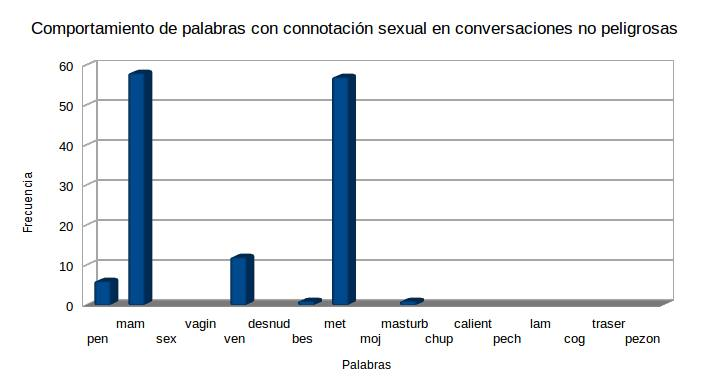
\includegraphics[scale=.4]{images/palabrassexuales1}
	\caption{Frecuencia de palabras de car\'acter sexual en conversaciones no peligrosas}
	\label{fig:graficasexual1}
\end{center}
\end{figure}


\begin{figure}[h]
\begin{center}
	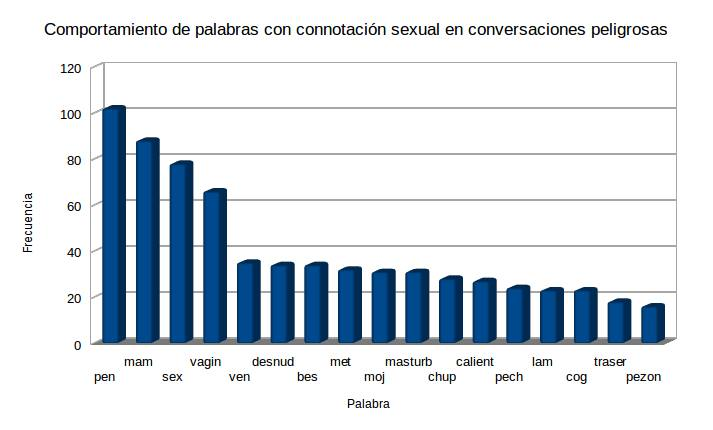
\includegraphics[scale=.4]{images/palabrassexuales2}
	\caption{Frecuencia de palabras de car\'acter sexual en conversaciones peligrosas}
	\label{fig:graficasexual2}
\end{center}
\end{figure}

\section{Descripci\'on}

Este prototipo genera vectores de frecuencia de las palabras del Nivel 5 de la matriz de caracterizaci\'on del comportamiento de conversaciones enfocadas al Online grooming.
\section{Objetivo}
Crear un prototipo que genere vectores de frecuencia de acuerdo al diccionario de palabras correspondientes al Nivel 5 de la matriz de frecuencias de la caracterizaci\'on del comportamiento de conversaciones enfocadas al Online grooming..

\section{An\'alisis}
\subsection{Caracter\'isticas}

\begin{description}
\item[FEAT1] El sistema recibe como entrada una conversaci\'on almacenada en un archivo de texto plano.
\item[FEAT2] El sistema recibe como entrada un archivo una conversaci\'on con un formato xml.
\item[FEAT2] Las palabras del diccionario son editables.
\item[FEAT3] El sistema genera el vector de frecuencias de acuerdo al diccionario dado.
\end{description}

\subsection{Restricciones}
\begin{itemize}
\item Persistencia de vectores en archivos.
\item Lenguaje de programaci\'on python.
\end{itemize}


\section{Dise\~no}

La figura \ref{fig:arquitectura_vector} muestra la arquitectura del comportamiento del prototipo, la cual recibe como entrada las conversaciones en formato plano o con formato xml y como salida se obtiene un vector asociado el cual representa la frecuencia de palabras que pertenecen al Nivel 5 de la matriz de caracterizaci\'on.

\begin{center}
	\begin{figure}[h]
		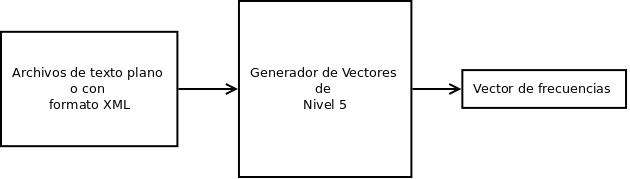
\includegraphics[scale=.5]{images/diagramavectores}
		\caption{Arquitectura Protipo 2}
		\label{fig:arquitectura_vector}
	\end{figure}
\end{center}


En la figura \ref{fig:diagramaActividades} se muestra el diagrama de actividades de la generac\'on de vectores del prototipo. En primer lugar se obtienen las conversaciones de las cuales queremos calcular el vector. El siguiente paso es ignorar palabras sin significado las cuales denominamos stopwords. Obtenemos la ra\'iz mediante el algoritmo de stemming de las palabras. Comparamos las palabras con el diccionario de palabras que tenemos del nivel 5, es decir, las palabras anteriormente listadas. Si la ra\'iz de la palabra que estamos analizando coincide con alguna de nuestro diccionario entonces aumentamos en 1 el valor de la componente del vector que est\'a asociada a dicha palabra.

	\begin{figure}[h]
	\begin{center}
		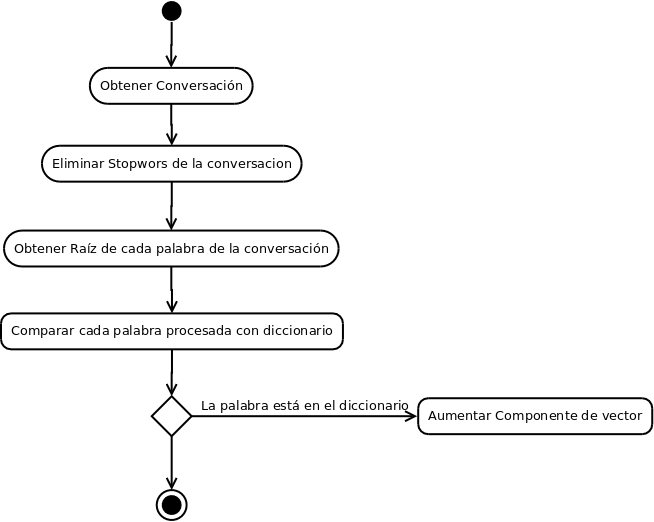
\includegraphics[scale=.35]{images/actividades_vectores}
		\label{fig:diagramaActividades}
		\caption{Diagrama de Actividades del Generador de Vectores}
		\end{center}
	\end{figure}


\section{Resultados}
\subsection{Pruebas}
El prototipo se probó con la generaci\'on de vectores de dimenciones de 3 componentes y 13 componentes.

Las componentes del primer tipo de vector est\'an asociadas al siguiente conjunto de palabras:
\begin{itemize}
\item Lista 1: desnudo, pene, vagina. 

Las componentes del segundo tipo de vector est\'an asociadas al siguiente conjunto de palabras:

\item Lista 2: chupar, coger, follar, lamer, besar, pene, vagina, masturbar, sexo, pechos, tetas, clitoris, tragar.
\end{itemize}

Para ambas listas de palabras se generaron los vectores correspondientes a 50 conversaciones extra\'idas del portal \url{http://www.perverted-justice.com/}, el cual, como ya se hab\'ia mencionado antes, es un sitio donde se hacen p\'ublicas conversaciones que han servido de anzuelo para capturar ped\'ofilos en internet. Estas conversaciones fueron traducidas al español y se anexan en el ap\'endice \ref{app:conversaciones}.


De igual manera se obtuvieron las caracter\'isticas de 50 conversaciones no peligrosas extra\'idas de conversaciones diarias de nuestras cuentas personales de Facebook anexadas en el aprendice \ref{app:conversacionesnp}.

La figura \ref{fig:graficaVectores} muestra la gr\'afica que contiene los vectores de 3 componentes generados por el prototipo. Marcados con puntos amarillos los vectores que representan la clase peligrosa, como podemos observar est\'an en el centro del plano. Mientras que las no peligrosas tienen una disperci\'on fuera del centro. 

Con esto podemos formular una hip\'otesis donde las conversaciones no peligrosas se posicionan en el origen del plano. Con esto podemos decir que este problema es linealmente separable cosa que nos ayudar\'a en la construcci\'on del clasificador. 

\begin{center}
\begin{figure}[h]
	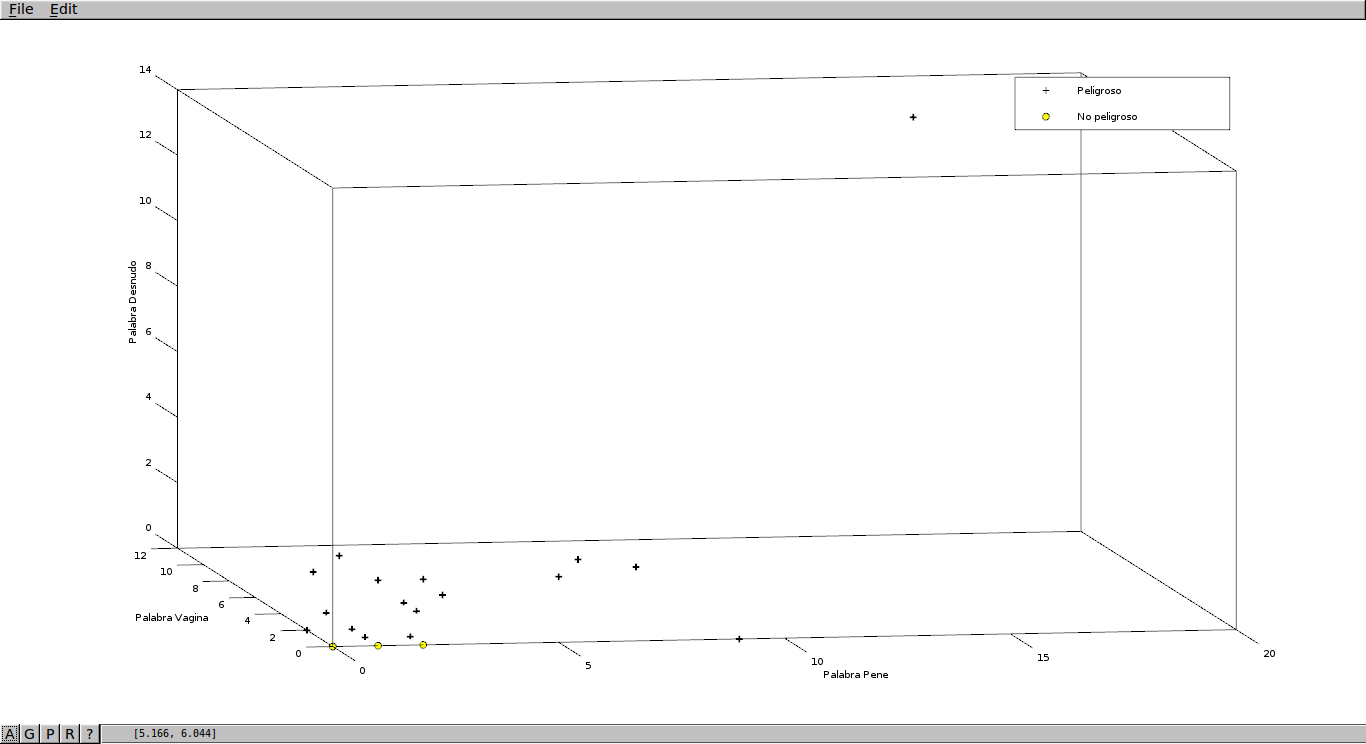
\includegraphics[scale=.3]{images/vectores}
	\caption{Gr\'afica de vectores generados}
	\label{fig:graficaVectores}
\end{figure}
\end{center}

Al aumentar el n\'umero de caracter\'iscas, esperamos que la separabilidad de las clases sea a\'un m\'as evidente por eso hemos seleccionado 13 caracter\'isticas para entrenar al clasificador del prototipo 3.
